\chapter{Public Transport in the UK}

\resp{Author name(s)...}


\section{Introduction}
    In this project we will create networks representing different cities in the United Kingdom that are made up of all public transport options that stay within that city. We utilise a dataset created by Riccardo Gallotti and Marc Barthelemy \cite{Gallotti2015} that integrates data from the timetables of all different types of public transport options in the UK to create a complete picture of all public transport options for a time period of a week in October 2010.
    The aim of this project is to recreate layered networks of public transport for UK cities. We will restrict our work to cities with at least 50k inhabitants \cite{worldpopReview2025} and, for each city, we will create two files; one for nodes and one for edges. With this data we will then construct our networks for all these cities.

\section{Method}
\subsection{Creating the Nodes and Edges Datasets}

    With the nodes, edges and the inhabitants of each UK city read from the initial data files we proceed with filtering the population data to just cities with at least 50k inhabitants. We then assign our nodes to one of those cities - we compare the longitude/latitude of each node with the longitude/latitude of each city centre and select the one closest to the node. If the node is further than 10km from any city centre then we leave it unassigned (left as NA).
    This adds a 'city' column in the nodes dataset - the city that the node is in. Once this is done for all nodes we loop through each city and create two datasets for the city's nodes and edges. The procedure for doing this is the following:

\begin{enumerate}
  \item First we run an if statement to only consider nodes where the city value is not NA.
  \item We then filter the nodes to include only those that are in the city we are looking at
  \item We also must get the edges that are within this city - these would be the edges that link between two nodes that are both within the relevant city. You can see we filter only for the edges where both the origin and destination nodes are both in the 'city nodes' dataset.
  \item With all the nodes and edges in the city accounted for we write two new .csv files for them both. Repeat for each city.
\end{enumerate}

\subsection{Constructing the Networks}

    With the data separated into different .csv files dependent on which city the nodes reside in we can move on to using these datasets to construct networks showing these journeys. We create a vector of colours to apply to the edges to represent the different transport options. These are:

\textcolor{yellow}{YELLOW} – Bus

\textcolor{cyan}{CYAN} – Coach

\textcolor{green}{GREEN} – Metro

\textcolor{blue}{BLUE} – Rail

\textcolor{purple}{PURPLE} – Ferry

\textcolor{red}{RED} – Air

We also create a new function called 'calculate relative coordinates'. This function takes values of longitude and latitude for a node and determines the displacement of the node from the city centre. We then convert this into cartesian coordinates so that it can be used effectively in the plotting.

Finally we use everything we have done to plot the networks for each city. We cycle through every relevant city and save the values for the longitude and latitude of the city centre. We then also load the city nodes and edges whilst also filtering out the edges that loop back to the same destination node as its origin node.

We run into an issue where the same node is used for each layer that it exists in (each layer represents the network of a singular transport option) so contracting all layers into one network would result in overlapping nodes where a stop/station services multiple transport options. To prevent this we aggregate all nodes with the same coordinates into one and and have all relevant edges connect to this node.

We now determine the relative coordinates of the nodes to the city centre and use these to plot our network. The networks for the cities can be visualised below. \cite{chatgpt2025}

\newpage

\vspace*{\fill} % Push content down

\begin{center}
  \begin{minipage}{0.45\textwidth}
    \centering
    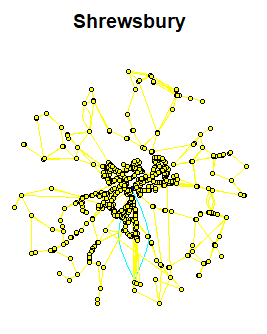
\includegraphics[width=\linewidth]{images/ShrewsburyMAP.png}
    \captionof{figure}{Transport map of Shrewsbury, which is an example of a standard map we'd seee in our dataset. The town centre has a dense bus network, the periphary has a sparse bus network, and a few long-range transport options are used to connect Shrewsbury to other towns (coach/train).}
    \label{fig:image1}
  \end{minipage}
  \hfill
  \begin{minipage}{0.45\textwidth}
    \centering
    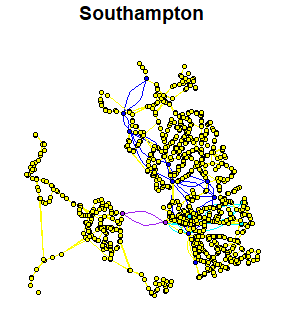
\includegraphics[width=\linewidth]{images/SouthamptonMAP.png}
    \captionof{figure}{Transport map for Southampton, a larger city on the south coast of England. I chose this partly because its familiar to me as my father lives here, but mainly for its unique ferry connection to the Isle of Wight, an island off the coast. The city itself is well connected to other cities through train and coach connections (I personally take the coach from London and then the ferry to the island), but the Isle of Wight has nothing except for buses. This map is an example of how natural obstacles can impact network topology and the types of permissable edges we can have between nodes}
    \label{fig:image2}
  \end{minipage}
\end{center}

\vspace*{\fill} % Push content up

\newpage

\vspace*{\fill} % Push content down

\begin{center}
  \begin{minipage}{0.45\textwidth}
    \centering
    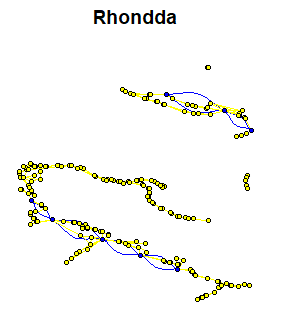
\includegraphics[width=\linewidth]{images/RhonddaMAP.png}
    \captionof{figure}{Transport map of Rhondda, a small Welsh town located within the Rhondda Valley in the Rhondda Cynon Taf mountain range. This town is another example of how natural, real world features can affect our network, this time due to mountain ranges that restricts the types of transport that can be used. We see as the network goes further into the real-world valley only buses remain as a realistic public transport option.}
    \label{fig:image1}
  \end{minipage}
  \hfill
  \begin{minipage}{0.45\textwidth}
    \centering
    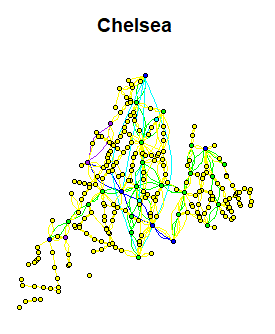
\includegraphics[width=\linewidth]{images/ChelseaMAP.png}
    \captionof{figure}{Transport map for Chelsea, a borough in London and an example of how areas of an incredibly large city are visualised in our dataset of maps. We see that, compared to other maps, there is an abundance of different transport options; the London Underground (metro), the Overground (trains), the ferry connections on the river Thames and the coaches that service the many coach stations in London. We also especially note the unique shape and smaller number of nodes - this effect is due to London boroughs are much closer together than towns and cities are, meaning they 'steal' nodes that otherwise would have gone to a 'city' like Chelsea. Chelsea was chosen in particular because it is where I went to school (and the location of the football team I support).}
    \label{fig:image2}
  \end{minipage}
\end{center}

\vspace*{\fill} % Push content up